% !TeX root = ../main.tex
% reduce display equation skip
 \setlength{\abovedisplayskip}{4pt}
 \setlength{\belowdisplayskip}{4pt}
 \setlength{\textfloatsep}{4pt}

We apply the calibration methods in \autoref{related} to image classification and document classification neural networks.
For image classification we use 6 datasets:
\begin{enumerate}[noitemsep,nolistsep]
\item Caltech-UCSD Birds \cite{cubdataset}: 200 bird species. 5994/2897/2897 images for train/validation/test sets.
\item Stanford Cars \cite{carsdataset}: 196 classes of cars by make, model, and year. 8041/4020/4020 images for train/validation/test.
\item ImageNet 2012 \cite{deng2009imagenet}: Natural scene images from 1000 classes. 1.3 million/25,000/25,000 images for train/validation/test.
\item CIFAR-10/CIFAR-100 \cite{krizhevsky2009learning}: Color images ($32\times 32$) from 10/100 classes. 45,000/5,000/10,000 images for train/validation/test.
\item Street View House Numbers (SVHN) \cite{netzer2011reading}: $32\times 32$ colored images of cropped out house numbers from Google Street View.
598,388/6,000/26,032 images for train/validation/test.
\end{enumerate}
%
We train state-of-the-art convolutional networks: ResNets \cite{he2015deep}, ResNets with stochastic depth (SD) \cite{huang2016deep}, Wide ResNets \cite{zagoruyko2016wide}, and DenseNets \cite{huang2016densely}. We use the data preprocessing, training procedures, and hyperparameters as described in each paper. For Birds and Cars, we fine-tune networks pretrained on ImageNet.

For document classification we experiment with 4 datasets:
\begin{enumerate}[noitemsep,nolistsep]
\item 20 News: News articles, partitioned into 20 categories by content. 9034/2259/7528 documents for train/validation/test.
\item Reuters: News articles, partitioned into 8 categories by topic. 4388/1097/2189 documents for train/validation/test.
\item Stanford Sentiment Treebank (SST) \cite{socher2013recursive}: Movie reviews, represented as sentence parse trees that are annotated by sentiment. Each sample includes a coarse binary label and a fine grained 5-class label.
As described in \cite{tai2015improved}, the training/validation/test sets contain 6920/872/1821 documents for binary, and 544/1101/2210 for fine-grained.
\end{enumerate}
On 20 News and Reuters, we train Deep Averaging Networks (DANs) \cite{iyyer2015deep} with 3 feed-forward layers and Batch Normalization.  On SST, we train \mbox{TreeLSTMs} (Long Short Term Memory) \cite{tai2015improved}.
For both models we use the default hyperparmaeters suggested by the authors.
%We leave more comprehensive empirical studies of calibration on RNNs to future works.

\begin{figure*}[h!]
	\centering
	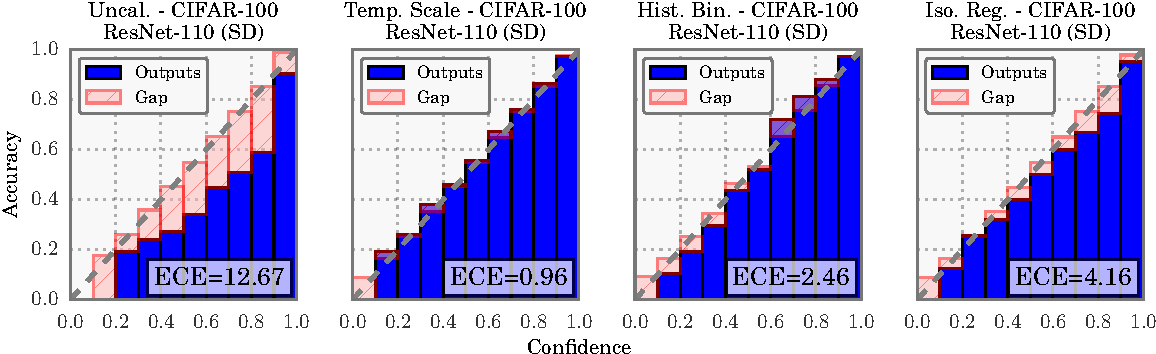
\includegraphics[width=0.98\textwidth]{fig/reliability-cifar100.pdf}
	\caption{Reliability diagrams for CIFAR-100 before (far left) and after calibration (middle left, middle right, far right).}
	\label{figure.reliability}
\end{figure*}

\paragraph{Calibration Results.}
\autoref{table.ece} displays model calibration, as measured by ECE (with $M=15$ bins), before and after applying the various methods (see \autoref{sup:tables} for MCE, NLL, and error tables).
It is worth noting that most datasets and models experience some degree of miscalibration, with ECE typically between $4$ to $10\%$.
This is not architecture specific: we observe miscalibration on convolutional networks (with and without skip connections), recurrent networks, and deep averaging networks.
 % problem problem of miscalibration is very pronounced on these recurrent neural networks. This is consistent with our observation that deeper networks tend to be less calibrated, as RNNs can be understood as extremely deep feed-forward networks~\cite{hochreiter1997long}.
The two notable exceptions are SVHN and Reuters, both of which experience ECE values below $1\%$. Both of these datasets have very low error ($1.98\%$ and $2.97\%$, respectively); and therefore the ratio of ECE to error is comparable to other datasets.

Our most important discovery is the \emph{surprising effectiveness of temperature scaling} despite its remarkable simplicity. Temperature scaling outperforms all other methods on the vision tasks, and performs comparably to other methods on the NLP datasets. What is perhaps even more surprising is that temperature scaling outperforms the vector and matrix Platt scaling variants, which are strictly more general methods. In fact, vector scaling recovers essentially the same solution as temperature scaling -- the learned vector has nearly constant entries, and therefore is no different than a scalar transformation. In other words, network miscalibration is intrinsically low dimensional.

The only dataset that temperature scaling does not calibrate is the Reuters dataset. In this instance, only one of the above methods is able to improve calibration. Because this dataset is well-calibrated to begin with (ECE $\leq 1\%$), there is not much room for improvement with any method, and post-processing may not even be necessary to begin with. It is also possible that our measurements are affected by dataset split or by the particular binning scheme.

% However, on Reuters, vector scaling performs considerably better than temperature scaling. We suspect this is due to class imbalance, as the network becomes overconfident about different classes at different rates. We investigated into this phenomenon by weighting the NLL loss by the inverse of class proportions, i.e. $$\scrL_{\rho}(\mathbf{x},\mathbf{y}) = -\sum_{i=1}^{n} \frac{\log(\hat{\pi}(y_i|x_i))}{\rho^{(y_i)}}$$ where $\rho^{(k)}$ is the proportion of class $k$ in the training set. By artificially balancing the classes this way, we find that temperature scaling performs similarly to vector scaling and the optimal scaling vector has equal entries once again.

Matrix scaling performs poorly on datasets with hundreds of classes (i.e. Birds, Cars, and CIFAR-100), and fails to converge on the 1000-class ImageNet dataset.
This is expected, since the number of parameters scales quadratically with the number of classes.
Any calibration model with tens of thousands (or more) parameters will overfit to a small validation set, even when applying regularization.

Binning methods improve calibration on most datasets, but do not outperform temperature scaling. Additionally, binning methods tend to change class predictions which hurts accuracy (see \autoref{sup:tables}). Histogram binning, the simplest binning method, typically outperforms isotonic regression and BBQ, despite the fact that both methods are strictly more general. This further supports our finding that calibration is best corrected by simple models.

\paragraph{Reliability diagrams.} \autoref{figure.reliability} contains reliability diagrams for 110-layer ResNets on CIFAR-100 before and after calibration. From the far left diagram, we see that the uncalibrated ResNet tends to be overconfident in its predictions. We then can observe the effects of temperature scaling (middle left), histogram binning (middle right), and isotonic regression (far right) on calibration. All three displayed methods produce much better confidence estimates. Of the three methods, temperature scaling most closely recovers the desired diagonal function. Each of the bins are well calibrated, which is remarkable given that all the probabilities were modified by only a single parameter. We include reliability diagrams for other datasets in \autoref{sup:reliability}.

\paragraph{Computation time.} All methods scale linearly with the number of validation set samples. Temperature scaling is by far the fastest method, as it amounts to a one-dimensional convex optimization problem. Using a conjugate gradient solver, the optimal temperature can be found in 10 iterations, or a fraction of a second on most modern hardware. In fact, even a naive line-search for the optimal temperature is faster than any of the other methods. The computational complexity of vector and matrix scaling are linear and quadratic respectively in the number of classes, reflecting the number of parameters in each method. For CIFAR-100 ($K=100$), finding a near-optimal vector scaling solution with conjugate gradient descent requires at least 2 orders of magnitude more time. Histogram binning and isotonic regression take an order of magnitude longer than temperature scaling, and BBQ takes roughly 3 orders of magnitude more time.

\paragraph{Ease of implementation.} BBQ is arguably the most difficult to implement, as it requires implementing a model averaging scheme.
While all other methods are relatively easy to implement, temperature scaling may arguably be the most straightforward to incorporate into a neural network pipeline.
In Torch7 \citep{collobert2011torch7}, for example, we implement temperature scaling by inserting a \texttt{nn.MulConstant} between the logits and the softmax, whose parameter is $1/T$.
We set $T\!=\!1$ during training, and subsequently find its optimal value on the validation set.\footnote{
  For an example implementation, see \url{http://github.com/gpleiss/temperature_scaling}.
}
